%%
%% This is file `thesis-ex.tex',
%% generated with the docstrip utility.
%%
%% The original source files were:
%%
%% uiucthesis.dtx  (with options: `example')
%% 
\def\fileversion{v1.0n} \def\filedate{1997/09/15}
%% Package "uiucthesis" for use with LaTeX2e.
\documentclass[12pt,oneside]{book}
%%\usepackage[draftthesis,fullpage]{uiucthesis}
\usepackage[fullpage]{uiucthesis}
\usepackage{graphics}
\usepackage{latexsym}
\usepackage{jeffe}

\begin{document}

\title{Lower Query Bounds in the Quantum Oracle Model}
\author{Matthew Joel Hayward}
\department{Computer Science}
\schools{B.S., University of Illinois at Urbana-Champaign, 2000\\
         B.S., University of Illinois at Urbana-Champaign, 2000}
\msthesis
\degreeyear{2002}
\maketitle

\frontmatter

%% Create a dedication with no heading, centered vertically
%% on the page.

\chapter*{Acknowledgments}

I am grateful for the support of Professor Jeff Erickson, without
whose time and insight this thesis never could have been written.  To
my parents, John and Linda Hayward, whose support and encouragement
have allowed me to pursue education: thank you.

%% The thesis format requires these lists to come in the following
%% order:
%%
%% Table of Contents
%% List of Tables
%% List of Figures or List of Illustrations
%% List of Symbols and/or Abbreviations

\tableofcontents
\listoftables
\listoffigures

%% Create a List of Abbreviations.

\chapter*{List of Abbreviations}
\begin{description}
\item[$A \times B$:] The Cartesian product of the sets $A$ and $B$.
\item[AND:] The Boolean function that returns 1 if and only if every input bit is 1.
\item[$D(f)$:] The decision tree complexity of the function $f$.
\item[$D(f,x)$:] The minimum number of bits of input $x$ that determine the value of $f(x)$.
\item[$D_{0}(f)$:] The nondeterministic decision tree complexity 
of verifying that $f(x) = 0$.
\item[$D_{1}(f)$:] The nondeterministic decision tree complexity 
of verifying that $f(x) = 1$.
\item[$N(f)$:] The nondeterministic decision tree complexity of the function $f$.
\item[OR:] The Boolean function that returns 0 if and only if every input bit is 0.
\item[PARITY:] The Boolean function that returns 1 if and only if the number of 1 bits in the input is even.
\item[MAJORITY:] The Boolean function that returns 1 if and only if more than half of the input bits are 1.


\end{description}


\mainmatter

\chapter{Introduction}
\label{ch:introduction}

The relatively new field of quantum computing has seen rapid growth in
the past two decades.  Quantum computing spans the theoretical and
applied sides of both computer science and quantum physics.  From its
beginnings as a thought experiment, its growth into formal system, and
finally its detailed analysis and construction, the development of
quantum computing has paralleled the early development of classical
computing.

In Section \ref{sec:mot} we briefly examine some of the reasons for
interest in quantum computing.  We then turn our attention to early
results and prominent quantum algorithms in Section \ref{sec:early}.
We review the theory and notation of quantum computing in Section
\ref{sec:quant}.  Following that we underline the importance of lower
bounds in Section \ref{sec:lower}, and summarize our results in
Section \ref{sec:sumofres}.

\section{Motivation}
\label{sec:mot}

\subsubsection{Possible Violation of the Polynomial Church-Turing Thesis}

One of the fundamental axioms of computer science is the Church-Turing
thesis, which states that any function computable by a ``realistic''
computer can be computed by a Turing machine.  An extension of the
Church-Turing thesis, the Polynomial Church-Turing thesis states:
\begin{quote}
\ldots any reasonable attempt to model mathematically
computer algorithms and their time performance is bound to end up with
a model of computation and associated time cost that is equivalent to
Turing machines within a polynomial \cite{papa94complexity}.
\end{quote} 
This says essentially that all physically realizable computing devices
are, within a polynomial factor, equivalent to one another in their
time complexity.

In the early 1980's physicist Richard Feynman observed that no
classical computer can simulate a quantum mechanical system of
particles without incurring exponential slowdown
\cite{williams98quantum}.  He also suggested that a computer that
behaves in a quantum-mechanical way could potentially simulate such
systems without exponential slowdown \cite{williams98quantum}.  The
possibility that a quantum computer could violate the polynomial
Church-Turning thesis made the study of quantum computation appealing,
and provided a strong incentive for studying quantum time complexity.
Many of the earliest problems and algorithms for quantum computers
were explicitly designed to show tasks that a quantum computer
performs exponentially faster than a classical Turing machine.
	
\subsubsection{Hardware Trends Toward Quantum Sizes}

Another strong incentive to study quantum computing is the
miniaturization of classical computing components.  The size of
transistors and memory elements has shrunk at an exponential rate.  At
the current rate, sometime around 2020 the number of atoms used to
represent a bit will be 1 \cite{williams98quantum}.  At this scale,
quantum mechanics will dominate the behavior of the memory element.
Whether or not quantum computing will provide a launch pad for a new
generation of computing devices is irrelevant to the practical need to
understand and manipulate systems so small that their behavior is
dictated by quantum physics.

\section{Early Results}
\label{sec:early}

\paragraph{Deutsch's Universal Quantum Computer:}
In 1985 David Deutsch published his seminal paper
\emph{Quantum theory, the Church-Turing principle and the universal
quantum computer} \cite{deutsch85quantum}.  In this paper Deutsch
defined a quantum generalization of the classical Turing machine,
showed that all Turing computable functions are also computable by his
universal quantum computer, and exhibited a task that his universal
quantum computer is more efficient for than any classical restriction
of it \cite{deutsch85quantum}.

Following this paper, researchers identified several toy problems that
a quantum computer is exponentially faster for than a classical Turing
machine \cite{brassard97exact} \cite{berthiaume92oracle}.
Unfortunately, these were all contrived problems with no practical
application.  While the potential for exponential speedup fostered
great curiosity, the study of quantum computing remained primarily
academic.

\subsubsection{Prominent Quantum Algorithms}

\paragraph{Shor's Algorithm:}
The status of quantum computing as a matter of academic curiosity
changed rapidly in 1994 when Peter Shor published his paper
\emph{Algorithms for Quantum Computation: Discrete Logarithms and
Factoring}.  The primary result of the paper was a polynomial time
quantum algorithm for factoring large integers
\cite{shor94algorithms}. It is not known if there is a classical
algorithm for factoring large integers efficiently, but the best
algorithms published thus far are exponential
\cite{williams98quantum}.  The presumed difficulty of factoring 
large integers is the basis for most modern cryptography.  The
importance of cryptography and its potential frailty in the face of
Shor's algorithm argue for earnestly researching the practicality of
constructing a quantum computer; this endeavor is currently ongoing in
multiple corporate, government, and academic research facilities
\cite{ibm01shor} \cite{chuang98quantum}.

\paragraph{Grover's Algorithm:}
In 1996 L. K. Grover published his paper \emph{A Fast Quantum
Mechanical Algorithm for Database Search} providing a $O(\sqrt{N})$
time algorithm for finding a single marked element in an unsorted
database of $N$ elements \cite{grover96fast}; the best possible
classical algorithm requires $\Omega(N)$ time.  This unordered search
problem was not the first problem for which a quantum algorithm was
shown to be asymptotically faster than any classical algorithm, but it
was the first such problem of real utility.  Grover's algorithm is
optimal to within a constant factor, so the potential speedup of any
quantum algorithm for the unordered search problem is moderate: a
quadratic factor.  While Shor's algorithm may be of more immediate
utility, Grover's algorithm seems more interesting in a theoretical
sense, as it highlights an area of fundamental superiority in quantum
computation.

\section{Quantum Computing}
\label{sec:quant}

The study of quantum computing is frequently opaqued by the demands
that it places on the investigator's sophistication in quantum
mechanics.  We try in this section to present the basics of quantum
computation and some common notation without delving deeply into
quantum physics.  For more detailed information the author suggests
\emph{Quantum Computation} by Andr\'{e} Berthiaume
\cite{berthiaume97quantum}.

\subsubsection{Bits and Qubits}

The most fundamental building block of the classical computer is the
bit.  A bit is a variable with only two possible values: 0 or 1.  The
smallest conceivable storage for a bit involves a single elementary
particle of some sort.  Consider a particle with a spin-1/2
characteristic that when measured is either $+1/2$ or $-1/2$.  We
could encode 1 to be $+1/2$ and 0 to be $-1/2$, and if we could
measure and manipulate the spin of such a particle, then we could
theoretically use this particle to store one bit of information.  The
spin-1/2 particle, or any two state system that behaves in a quantum
manner, could instead be the fundamental building block of a quantum
computer.  We will call a two state quantum system a \emph{qubit}, to
denote that it is analogous to a classical bit.  When a classical bit
is measured, the value observed will always be the value stored.
Quantum physics states that when we measure a qubit we will find it in
one of two states, which we can label 0 and 1.  The differences
between the qubit and the bit arise from the possible state of a qubit
between measurements.

\subsubsection{State Vectors and Dirac Notation}

To quantify the state of our qubit when it is not being measured, we
introduce the concept of the \emph{state vector}, which will
completely describe the state of our qubit, and later the state of a
quantum register which we construct from multiple qubits.

\paragraph{State Vectors:} 
We can describe the state of any quantum system by a state vector in a
Hilbert space.  A Hilbert space is a complex linear vector space
$\Complex^{N}$ \cite{williams98quantum}.  In the Hilbert space for a
state vector describing an $N$-state quantum system there will be $N$
perpendicular axes, which correspond to the measurable states of the
system.  These are called basis states or \emph{eigenstates}.  In
general, the total state of a quantum system can be any complex linear
combination of the basis states.  The Hilbert space for a single qubit
has two perpendicular axes, one corresponding to the 0 state, and the
other corresponding to the 1 state.

\paragraph{Dirac Notation:}

The standard notation for a state vector is a \emph{ket vector}
$|\Psi\rangle$.  For example, a vector in $\Real^{3}$ with basis
$\hat{i},\hat{j},\hat{k}$ is typically written as
\[
\vec{v} =  a\hat{i}  +  b\hat{j}  +  c\hat{k}  =  (a,b,c)^{T} .
\]
In Dirac notation, it would be written as
\[
|v\rangle  =  a|i\rangle  +  b|j\rangle +  c|k\rangle  = 
(a,b,c)^{T}. 
\]
The term ket and this notation come from the physicist Paul Dirac who
wanted a concise way of writing formulas involving row and column
vectors.  He referred to row vectors as \emph{bra vectors} represented
as $\langle y|$.  The inner product of a \emph{bra} and a \emph{ket}
vector is written $\langle y|x\rangle$, and is called a \emph{bracket}
\cite{williams98quantum}.

\subsubsection{Superposition}

The projection of the state vector onto one of the axes of its Hilbert
space shows the contribution of that axis's eigenstate to the whole
state.  A classical bit's state vector can only lie along one of the
two axes.  The state of a qubit can be any vector $|X\rangle$ in the
Hilbert space with $\langle X|X\rangle = 1$; such a state vector is
called \emph{normalized}.  The inner product of a vector $|X\rangle =
(x_{0},x_{1},\ldots, x_{N-1})^{T}$ with itself is $|x_{0}|^{2} +
|x_{1}|^{2} + \ldots + |x_{N-1}|^{2}$, where $|a+ib|^{2} = a^{2} +
b^{2}$.  More generally $\left\langle X|Y\right\rangle = \sum_{i =
0}^{N-1} x_{i}^{*}y_{i}$, where $(a + ib)^{*}$ is $a - ib$.

Let $x_{1}$ be the eigenstate corresponding to the 1 state, and let
$x_{0}$ be the eigenstate corresponding to the 0 state.  We can write
any state $|X\rangle$ as $w_{0}|x_{0}\rangle + w_{1}|x_{1}\rangle$,
where $w_{0}, w_{1}$ are the complex projections of $|X\rangle$ onto
the eigenstates such that $|w_{0}|^{2} + |w_{1}|^{2} = 1$.  When the
qubit with state vector $X$ is measured, we are guaranteed to find it
to be in either the state $1 |x_{0} \rangle + 0 |x_{1} \rangle =
|x_{0}\rangle$ or the state $0 |x_{0} \rangle + 1 |x_{1} \rangle =
|x_{1}\rangle$.

More generally, the Hilbert space of an $N$-state quantum system is
$\Complex^{N}$.  As with the two state system, when we measure our
$N$-state quantum system we will always find it to be in exactly one
of the eigenstates.  The system is allowed to exist in any complex
linear superposition of the $N$ states between measurements.  An
$N$-state quantum system with eigenstates $x_{0}, x_{1},\ldots,
x_{N-1}$ can be fully described by the vector
\[|X \rangle = \sum_{k = 0}^{N-1} w_{k} |x_{k} \rangle, 
\textrm{ where }
\sum_{k = 0}^{N-1} |w_{k}|^{2} = 1.
\]

Our state vector can exist in a linear superposition of eigenstates,
but we can only measure the state vector to be in one of the
eigenstates.  When the state vector is observed, it makes a sudden
discontinuous jump to one of the eigenstates.  When measurement is
performed the state vector is said to collapse
\cite{williams98quantum}.  For an $N$-state quantum system with a 
normalized state vector, the probability that the state vector will
collapse into the $j$th eigenstate is simply $|w_{j}|^{2}$.  The
coefficient $w_{j}$ is called the \emph{amplitude} of eigenstate
$|x_{j}\rangle$.

We can construct a quantum memory register out of the qubits described
in the previous section.  Just as in a classical computer, a quantum
computer will perform calculations by manipulating its memory register
from some start state to some final state.  Note that a quantum
register composed of $N$ qubits requires $2^{N}$ complex numbers to
completely describe its state vector, as an $N$-qubit register has
$2^{N}$ basis states.

\subsubsection{Unitary Operators}

Not all functions on a quantum memory register preserve the
superposition of the state vector.  For example, measurement destroys
the superposition in the register.  Operations that collapse the state
vector are called \emph{measurements}, and any complex linear
transformation of the state vector is called an
\emph{operator}.  We can represent any operator on an $N$-bit 
quantum memory register in $\Complex^{2^{N}}$ as a matrix
\[T = \left( \begin{array}{cccc}
	T_{00} & T_{01} & \ldots & T_{0(2^{N}-1)} \\ T_{10} & T_{11} &
	\ldots & T_{2(2^{N}-1)} \\ \vdots & \vdots & & \vdots \\
	T_{(2^{N}-1)0} & T_{(2^{N}-1)1} & \ldots &
	T_{(2^{N}-1)(2^{N}-1)}
\end{array}\right) \] 
\cite{griffiths95quantum}.

Quantum mechanics imposes conditions on which linear transformations
are legal operators.  In particular, the operation must be reversible,
and it must preserve the length of the state vector
\cite{griffiths95quantum}.  If we impose the condition that the sum of
the kinetic and potential energy (called the Hamiltonian) of our
quantum memory register is constant, then all legal operators have
\emph{unitary} matrix representations.  A matrix $T$ is unitary if the
transpose of its complex conjugate is $T^{-1}$
\cite{griffiths95quantum}.  Systems with time-dependent Hamiltonians 
are not required to perform either Grover's or Shor's algorithm, and
are not within the scope of this thesis.

\subsubsection{Quantum Algorithms}
An operator taking a register in a superposition of states as an input
performs a ``computation'' on each of the components of the
superposition simultaneously.  Since the number of possible superposed
states is $2^{N}$ for an $N$-qubit register, in some sense a quantum
computer can perform in one operation what would take an exponential
number of operations on a classical computer.  Unfortunately, the more
superposed states, the smaller the probability that we will measure
the value of our function for any particular one.  Some clever
algorithms, most notably by Peter Shor and L. K. Grover, succeed by
considering a function for which some property of all the inputs is
useful.

A quantum memory register is just a state machine whose state
transitions are defined by the operators we apply.  A reversible
deterministic state machine with $2^{N}$ states can be modeled by an
$N$-bit register and operators which are $2^{N} \times 2^{N}$
permutation matrices.  A classical probabilistic state machine can be
modeled in a similar manner, as an $N$-bit register with a normalized
state vector in $\Real^{2^{N}}$ and operators that are doubly
stochastic matrices.  The difference between the quantum computer and
the probabilistic computer is that the projection of the quantum state
vector onto any eigenstate is a complex number: it has both a
magnitude and a phase.  The classical probabilistic state vector's
projection onto its eigenstates has only a positive real magnitude.
The amplitude of the quantum state vector allows for operators which
cause wave-like interference of the eigenstates, enforcing correct
solutions and diminishing incorrect ones
\cite{grover00search}.  

A quantum algorithm is described by an initial normalized state and a
sequence of unitary matrices representing linear transformations of
the state vector.  These unitary matrices should increase the
probability that the state vector collapses into a correct solution
state when measured.

\subsection{Error Models}
\label{sec:error}

Quantum computation is probabilistic in nature.  We must therefore
consider what (if any) error we will accept from our quantum
algorithms.  Different settings allow different expected running
times, just as in the classical case, where different running times
can be found for different types of randomized algorithms.

Three primary settings for quantum algorithms are defined by Beals et
al.\ \cite{beals98quantum}:
\begin{enumerate}

\item \textbf{The Exact Setting:} 
The quantum algorithm is required to return $f(x)$ with certainty for
every $x \in \{0,1\}^{N}$.

\item \textbf{The Zero Error Setting:}
The quantum algorithm may be inconclusive with probability at most
$1/2$, but if it returns an answer, it must be correct.

\item \textbf{The Bounded Error Setting:}
The quantum algorithm is required to return $f(x)$ with probability at
least $2/3$ for every $x \in \{0,1\}^{N}$ .
\end{enumerate}

Clearly any algorithm in the exact setting is also correct in the
bounded error setting.  Algorithms in the zero error setting can be
placed in the bounded error setting by performing multiple runs that
return an arbitrary value whenever they would return ``inconclusive.''
Thus the bounded error setting is the broadest category, and as such
offers the best potential speedups.  All the results in this thesis
refer to computations in the bounded error setting.

\section{Lower Bounds}
\label{sec:lower}

Given that we can theoretically attain exponential speedup through
quantum parallelism, it is tempting to hope that quantum computing
could offer exponential speedup to large classes of problems.  Shor's
algorithm seems to validate that hope.  The optimality of Grover's
algorithm, on the other hand, essentially establishes that a quantum
computer can offer at most quadratic speedup to the brute force
solution of a problem that exhaustively searches all possible
solutions.

To answer questions surrounding the power of the quantum computer, we
study lower bounds for quantum algorithms.  Lower bounds on large
classes of functions allow us to make quantitative comparisons between
quantum and classical computers.  It is very difficult to prove a
lower bound on a particular problem in any general model of
computation, as one has to argue how quickly any possible algorithm
can solve the problem.  Throughout this thesis we will consider a
restricted model of computation, the \emph{oracle query model}, in
which we consider only algorithms whose input is provided in a black
box.

We will present a theorem by Andris Ambainis that enables us to easily
prove lower bounds in the oracle query model
\cite{ambainis00quantum}.  The main strength of Ambainis' Theorem
is its ability to prove lower bounds for a variety of Boolean
functions, and thus allow us to compare the relative power of
classical and quantum computers.

\section{Summary}
\label{sec:outline}

In Chapter \ref{ch:oracle}, we define the quantum oracle model, and
present Ambainis' Theorem for proving lower bounds within this
framework.  We examine a shortcoming of Ambainis' Theorem, and then
derive two theorems and use them to prove lower query bounds for
symmetric functions.

In Chapter \ref{ch:graph}, we apply the results of Chapter
\ref{ch:oracle} to the interesting and well studied case of
non-trivial monotone graph properties.  Finding the results wanting we
appeal directly to Ambainis' Theorem to establish new lower bounds for
graph connectivity and bipartiteness.  Finally we show there is no
quantum extension of the Aanderaa-Karp-Rosenberg conjecture in the
bounded error setting.

In Chapter \ref{ch:general}, we examine classes of functions that do
not have the inherent symmetries of those in chapters \ref{ch:oracle}
and \ref{ch:graph}.  We provide lower query bounds for tree functions,
nondeterministically evasive functions, and sensitive functions.

We conclude in Chapter \ref{ch:open} with a brief examination of some
open questions for lower oracle query bounds in the bounded error
setting, and quantum computing in general.

\label{sec:sumofres}

Many of the results in this thesis have been attained previously by
other authors. We present these results again to illustrate how
Ambainis' Theorem can provide relatively simpler proofs for a variety
of problems.  Table \ref{tbl:results} summarizes our results and
credits previous papers where appropriate.  All results are in the
quantum bounded error setting.

\begin{table}
\begin{center}
\begin{tabular}{|l|l|l|l|}
\hline
Function & Lower Query Bound & Section & Reference \\ 
\hline
Generalized XOR & $\Omega\left(\sqrt{N}\right)$ & \ref{sec:gXOR} &  \\
\hline
Determining the Oracle String & $N/2$ & \ref{sec:dos} &  \\
\hline
Singleton functions & $\Omega\left(\sqrt{N}\right)$ & \ref{sec:torf1} & \\
\hline
Partially symmetric & $\Omega\left(\sqrt{\frac{(N-a)b}{(b-a)^{2}}}\right)$ & \ref{sec:lqbsym} &  \\
\hline
AND & $\Omega\left(\sqrt{N}\right)$ & \ref{sec:AOMP} & Beals et al.\ \cite{beals98quantum} \\
\hline
OR & $\Omega\left(\sqrt{N}\right)$ & \ref{sec:AOMP} & Beals et al.\ \cite{beals98quantum} \\
\hline
MAJORITY & $\Omega\left(N\right)$ & \ref{sec:AOMP} & Beals et al.\ \cite{beals98quantum} \\
\hline
PARITY & $\Omega\left(N\right)$ & \ref{sec:AOMP} & Beals et al.\ \cite{beals98quantum} \\
\hline
Nonconstant symmetric & $\Omega\left(\sqrt{N}\right)$ & \ref{sec:lqbnsf} & Beals et al.\ \cite{beals98quantum} \\
\hline
Graph connectivity & $\Omega\left(V\right)$ & \ref{sec:gc} & \\
\hline
Graph bipartiteness & $\Omega\left(V\right)$ & \ref{sec:bip} & \\
\hline
Tree functions & $\Omega\left(\sqrt[4]{N}\right)$ & \ref{sec:tree} & Beals et al.\ \cite{beals98quantum} \\
\hline
Nondeterministically evasive & $\Omega\left(\sqrt{N}\right)$ & \ref{sec:b4r} &  \\
\hline
Sensitive functions & $\Omega\left(\sqrt[4]{D(f)}\right)$ & \ref{sec:lqbcbf} & \\
\hline
\end{tabular}
\end{center}
\caption{Summary of Results \label{tbl:results}}
\end{table}

\newtheorem{theorem}{Theorem}[section]
\newtheorem{lemma}{Lemma}[section]
\newtheorem{defi}{Definition}[section]
\newtheorem{corollary}{Corollary}[section]

\chapter{Lower Oracle Query Bounds}
\label{ch:oracle}

In this chapter we present the quantum oracle framework.  We first
define the quantum oracle model and oracle query complexity, then
present a general theorem due to Ambainis \cite{ambainis00quantum}.
In Section \ref{sec:lplqb} we derive a key lemma used throughout the
thesis and apply it to a simple problem.  We then show that for the
problem of determining the oracle string, Ambainis' Theorem can not
attain an asymptotically tight lower query bound in Sections
\ref{sec:dos} and \ref{sec:torf1}.

Our primary purpose is to demonstrate the power and flexibility of
Ambainis' Theorem in attaining lower bounds on broad classes of
Boolean functions and simplifying previous proofs.  We investigate
Boolean functions with partial symmetry in Section \ref{sec:lqbsym}.
We apply the result of that section to attain asymptotically tight
lower oracle query bounds of $\Omega(\sqrt{N})$, $\Omega(\sqrt{N})$,
$\Omega(N)$, and $\Omega(N)$ for the functions AND, OR, MAJORITY, and
PARITY respectively in Section
\ref{sec:AOMP}.  Finally we prove $\Omega(\sqrt{N})$ oracle
queries are required to compute any $N$-bit nonconstant symmetric
Boolean function in Section \ref{sec:lqbnsf}.

\section{Preliminaries}

\subsubsection{Useful Definitions}

We will prove lower bounds for functions from $\{0,1\}^{N}$ to
$\{0,1\}$, we will call such functions \emph{$N$-bit Boolean
functions}, or just \emph{Boolean functions}.  In our proofs we will
frequently need the notion of the \emph{Hamming weight} of a bit
string: this is the number of 1's in the string.  We denote the
Hamming weight of a bit string $x$ as $|x|$.  We also will frequently
refer to all inputs which differ from a particular input in only one
bit, we will call inputs which differ in a single bit \emph{Hamming
neighbors}.

\subsubsection{Quantum Oracle Models}
\label{sec:qom}

In the quantum oracle model, we have an oracle that holds an $N$-bit
input string.  Our task is to determine the value of some fixed
Boolean function of the oracle string, using as few oracle queries as
possible.  An oracle query is a question of the form: ``What is the
$i$th bit of the oracle string?''  The quantum oracle model is a
special case of Ambainis' more general quantum adversary model
\cite{ambainis00quantum}, which we describe below.

In the quantum adversary model, we run an algorithm against an oracle
that contains a superposition of inputs.  Let $S$ be a subset of the
possible inputs $\{0,1\}^{N}$.  Algorithms in the quantum adversary
model will work in the Hilbert space $H = H_{A} \otimes H_{I}$, where
$H_{A} = \Complex^{2^{m}}$ is the Hilbert space of our $m$-qubit
memory register, and $H_{I} = \Complex^{|S|}$ is the Hilbert space
spanned by basis vectors $|x\rangle$ corresponding to the elements of
$S$.  We think of $H_{A}$ as our algorithm space, and $H_{I}$ as our
input space.  The tensor product of two vector spaces $A$ and $B$,
denoted $A \otimes B$, is a new vector space spanned by all possible
pairs $(i,j)$ of basis vectors $i$ from the first space and $j$ from
the second space. Thus $H = \Complex^{|S|2^{m}}$.

We can represent the basis states of our algorithm space as $|i, b,
z\rangle$, where $i$ consists of $\lceil\log{N}\rceil$ bits, $b$ is a
single bit, $z$ denotes all other bits our quantum algorithm requires.
We define the oracle transformation $O$ as the unitary operator that
takes any eigenstate $|i,b,z\rangle \otimes |x\rangle$ to $|i, b
\oplus x_{i}, z\rangle \otimes |x\rangle$. The first 
$\lceil\log{N}\rceil$ bits of the subspace defined by a particular
input $|x\rangle$ is the index $i$ to the oracle bit $x_{i}$ that we
are querying. $O$ is a permutation matrix.

A quantum algorithm that performs $T$ queries is just a sequence of
unitary transformations
\[U_{0}\rightarrow O\rightarrow U_{1} \rightarrow O \ldots \rightarrow U_{T-1} \rightarrow O \rightarrow U_{T},\]
where $U_{i}$ is an arbitrary unitary transformation that does not
depend on the oracle, and $O$ is the oracle transformation.  (Recall
that unitary transformations are reversible and preserve the
normalization of the state vector.)

The standard oracle query model is just an instance of the quantum
adversary model where the input space is spanned by a single
eigenstate $|x\rangle$.  In this case a quantum algorithm starts with
the state $|0\rangle \otimes |x\rangle$, applies $U_{0}, O, U_{1},
\ldots, O, U_{T}$, and then measures the final state.  The rightmost
bit of the measured state of the algorithm space is the output of the
algorithm on $x$.  The algorithm computes $f$ in the bounded error
setting if for every input $x \in \{0,1\}^{N}$, the output is $f(x)$
with some constant probability.

The measure of complexity in both the quantum oracle model and quantum
adversary model is the number of oracle queries.  It should be noted
that querying the oracle is not always the most time consuming portion
of an algorithm.  For example, to factor an $N$ bit integer that the
oracle holds, we can determine the integer in $N$ queries.  However,
we must then do $2^{N^{\Omega(1)}}$ additional steps in the classical
case, or $N^{2}\log^{O(1)}{N}$ additional steps in the quantum case to
factor the number using the best known algorithms
\cite{beals98quantum}. Nonetheless we restrict our attention to the 
number of oracle queries required, as it is clearly a lower bound on
the overall running time of the algorithm.  Classical bounds for query
complexity are well studied, making comparisons between quantum and
classical oracle query complexity possible.

\subsubsection{A Lower Query Bound Proving Framework due to Ambainis} 

Ambainis \cite{ambainis00quantum} proved the following fundamental
result:

\begin{theorem}[Ambainis]
\label{th:amb}
Let $f$ be an $N$-bit Boolean function and let $X$ and $Y$ be two sets
of inputs such that $f(x) \neq f(y)$ whenever $x \in X$ and $y \in Y$.
Let $P \subseteq X \times Y$ be a relation between $X$ and $Y$ with
the following properties:

\begin{enumerate}

\item
Every element of $X$ is related to at least $m$ elements of $Y$ by
$P$.

\item 
Every element of $Y$ is related to at least $m'$ elements of $X$ by
$P$.

\item 
For all $i$, every element $x \in X$ is related to at most $l$
elements $y \in Y$ such that $x_{i} \neq y_{i}$

\item 
For all $i$, every element $y \in Y$ is related to at most $l'$
elements $x \in X$ such that $x_{i} \neq y_{i}$

\end{enumerate}

Then
\[\Omega\left(\sqrt{\frac{mm^{\prime}}{ll^{\prime}}}\right)\] 
oracle queries are required by any quantum algorithm to compute $f$ in
the bounded error setting.
\end{theorem}

This theorem will be the primary means of proving lower bounds in this
thesis.  Its appeal is twofold; first, it leads to reasonably simple
proofs, and second, it unifies many existing lower bounds into a
single framework.

\paragraph{The Quantum Adversary:}

Lower bounds for both classical and quantum algorithms have been
attained in the past by analyzing the behavior of the algorithm in the
face of an adversary.  Ambainis uses a \emph{quantum adversary} as the
basis for his lower bound theorem; instead of running a quantum
algorithm against one input, it is run against a superposition of
inputs.  The formulation of the quantum adversary and the
justification for why a lower bound in the quantum adversary model is
also a lower bound in the standard oracle query model below are
adapted and somewhat simplified from Ambainis' paper
\cite{ambainis00quantum}.

Ambainis observed that any standard oracle query algorithm $A$ that
operates only on a single input is also correct in the quantum
adversary model.  Consider a standard oracle query algorithm $A$ that
uses $T$ queries and succeeds with probability $p$.  We assume our
quantum memory register begins in the $\left| 0 \right\rangle$ state.
For every input $x \in \{0,1\}^{N}$, the algorithm transforms the
initial state $\left| 0 \right\rangle \otimes \left| x \right\rangle$
into the final state
\[
\left(
  \alpha_{x}\left|f(x)\right\rangle
  +
  \beta_{x}|\overline{f(x)}\rangle
\right)
\otimes
\left|w_{x}\right\rangle
\otimes
\left|x\right\rangle
\]
where $|\alpha_{x}|^{2} + |\beta_{x}|^{2} = 1$, and $|\alpha_{x}|^{2}
\ge p$ (so $|\beta_{x}|^{2} \le 1-p$, and finally $|w_{x}\rangle$ is 
the remaining state of the memory. The same algorithm will take any
superposed input state
\[|0\rangle \otimes \sum_{x \in S} \frac{1}{\sqrt{\left|S\right|}} 
\left| x \right\rangle\]
to the final state
\[\frac{1}{\sqrt{|S|}} \sum_{x \in S} 
\left(
  \alpha_{x}\left|f(x)\right\rangle
  +
  \beta_{x}|\overline{f(x)}\rangle
\right)
\otimes
\left|w_{x}\right\rangle
\otimes
\left|x\right\rangle.
\]
Note that in this end state, if the oracle is measured to be $x$, a
measurement of the memory register will yield $f(x)$ with probability
$|\alpha_{x}|^{2} \ge p$.  Ambainis places a lower bound on the number of
oracle queries required by any quantum adversary algorithm to produce
such an end state from such a start state.

This argument gives us a lower bound in the standard oracle query
model as well.  If $T$ queries are required of a quantum adversary
algorithm to establish a correct end state with probability $p$, then
no standard oracle query algorithm $A$ can compute $f$ with bounded
probability $p$ in $t < T$ queries. 

This quantum adversary method provides a framework for proving a great
diversity of lower bounds.  Indeed, nearly every lower bound in this
thesis is proved directly or indirectly using Theorem \ref{th:amb}.
As useful as the theorem is, it does have limitations, one of which is
discussed in Section \ref{sec:torf1}.

\section{A Lemma for Proving Lower Query Bounds}
\label{sec:lplqb}

The sensitivity of an input $x$ of a function $f$ is the number of
Hamming neighbors $y$ of $x$ such that $f(x) \neq f(y)$.  We will use
the following lemma to establish lower bounds for functions based
solely on their sensitivity for a particular input.

\begin{lemma}
\label{lm:1xky}
Let $f$ be an $N$-bit Boolean function.  If some input $x$ has $k$
Hamming neighbors $y$ such that $f(x) \neq f(y)$, then
$\Omega(\sqrt{k})$ oracle queries are required to compute $f$ in the
bounded error setting.
\end{lemma}

\begin{proof}
To prove Lemma \ref{lm:1xky} we will apply Theorem \ref{th:amb}.  Let
$X$ contain the single input $x$ from the statement of the lemma.  Let
$Y$ contain the $k$ Hamming neighbors of $x$ such that $f(x)
\neq f(y)$ when $y \in Y$.  Let $P$ be the complete relation from $X$
to $Y$.

Then $m = k$, since $xPy$ for each of the $k$ elements $y \in Y$.
Since no two Hamming neighbors of $x$ differ from $x$ in the same bit
position, we have $l = 1$.  Since there is only one element $x$ in $X$
and $xPy$ for each $y \in Y$, we have $m^{\prime} = l^{\prime} = 1$.
The result now follows immediately from Theorem \ref{th:amb}.
\end{proof}

This lemma will not in general provide us with the best lower bound
that can be attained from Ambainis' Theorem \ref{th:amb}: we are
maximizing $m/l$, but we make no attempt to maximize
$m^{\prime}/l^{\prime}$.  The strongest results of Ambainis' Theorem
frequently arise from maximizing both.  We will maximize both when
dealing with partially symmetric functions in Theorem \ref{th:ptsym}
and graph connectivity in Theorem \ref{th:gc}.  The \emph{singleton}
class of functions described in Sections \ref{sec:dos} and
\ref{sec:torf1} is a class for which Lemma \ref{lm:1xky} obtains 
optimal results.

\subsection{Application to Generalized XOR} 
\label{sec:gXOR}

To see how simple proofs can be with Lemma \ref{lm:1xky} we provide an
example.  Generalized XOR is the $N$-bit Boolean function that is 0 if
and only if its input bits are all the same.

\begin{theorem}
\label{th:gXOR}
$\Omega(\sqrt{N})$ oracle queries are required to compute
the generalized XOR of $N$ bits in the bounded error setting.
\end{theorem}

\begin{proof}
The generalized XOR of $0^{N}$ is $0$, and the generalized XOR of the
$N$ Hamming neighbors of $0^{N}$ is 1.  The theorem follows from Lemma
\ref{lm:1xky} with $k = N$.
\end{proof}

This lower bound is asymptotically tight: Beals et al.\ provide
$O(\sqrt{N})$ oracle query algorithms for computing the AND or OR of
$N$ bits in the bounded error setting \cite{beals98quantum}, and the
generalized XOR of $N$ bits is just $\overline{AND \vee
\overline{OR}}$.  Unfortunately, Ambainis' Theorem does not always 
perform this well, as we demonstrate in the next two sections.

\section{Determining the Oracle String}
\label{sec:dos}

Consider the problem of determining the oracle string.  We prove two
lower bounds for this problem, one through Lemma $\ref{lm:1xky}$, and
another by using a known lower bound for PARITY.

\begin{theorem}
\label{th:dosbad}
$\Omega(\sqrt{N})$ oracle queries are required to determine an $N$-bit
oracle string in the bounded error setting.
\end{theorem}

\begin{proof}
Let $f$ be the $N$-bit Boolean function that is 1 if and only if its
input is the same as the oracle string $x$.  For each Hamming neighbor
$y$ of $x$, we have $f(x) \neq f(y)$.  The result then follows from
Lemma \ref{lm:1xky}.
\end{proof}

In the classical case $N$ oracle queries are required to determine the
oracle string.  If the lower bound of $\Omega(\sqrt{N})$ oracle
queries were asymptotically tight, then there would be quadratic
improvement over the classical case for this problem.  This seems
plausible in light of Grover's algorithm.  However, $\Omega(N)$ lower
bounds are known for Boolean functions in the quantum oracle model, we
can thus infer that Theorem \ref{th:dosbad} is not asymptotically
tight.

\begin{theorem}
\label{th:dosgood}
$N/2$ oracle queries are required to determine an $N$-bit oracle
string in the bounded error setting.
\end{theorem}

\begin{proof}
Once we compute the oracle string, we can compute its PARITY with no
additional queries.  Beals et al.\ proved that $N/2$ oracle queries
are required to compute PARITY for an $N$-bit oracle string in the
bounded error setting \cite{beals98quantum}.
\end{proof}

We now see an apparent limitation of Ambainis' Theorem; the result
attained was quadratically worse than the asymptotically tight lower
bound.  We will show in the next section that the weak lower bound in
Theorem \ref{th:dosbad} is indeed the best that can be attained
through application of Ambainis' Theorem.

\section{Singleton Functions}
\label{sec:torf1}

An $N$-bit Boolean function that evaluates to 1 for exactly one input
is a singleton function.  We will show that for any $N$-bit singleton
function Ambainis' Theorem can always attain a lower query bound of
$\Omega(\sqrt{N})$, but no better.

The proof of the $\Omega(\sqrt{N})$ lower query bound for determining
the oracle string in Theorem \ref{th:dosbad} can equally well be
applied to any singleton function.

\begin{corollary}
\label{th:1sqn}
$\Omega(\sqrt{N})$ oracle queries are required to compute any $N$-bit
singleton function in the bounded error setting.
\end{corollary}

\begin{theorem}
\label{th:best}
$\Omega(\sqrt{N})$ is the best lower bound on the number of oracle
queries required to compute an $N$-bit singleton function that can be
attained from Theorem \ref{th:amb}.
\end{theorem}

\begin{proof}
We will consider every possible choice of $X$, $Y$, and $P$ in Theorem
\ref{th:amb}.

Without loss of generality, let $X$ contain the single input $x$ such
that $f(x) = 1$.  Let $Y$ be any subset of the $2^{N} - 1$ bit strings
for which $f(y) = 0$.  If $P$ is not the complete relation $X \times
Y$ then some element $y \in Y$ is not related to $x$ by $P$, so the
$m^{\prime}$ component of Theorem \ref{th:amb} is $0$, giving a
vacuous lower bound.  Thus $P$ is the complete relation.

Here $m = |Y|$, and $m' = l' = 1$.  The final parameter $l$ is the
maximum over all $i$ of the number of $y \in Y$ that differ from $x$
in the $i$th bit position.

From Ambainis' Theorem $\Omega(\sqrt{m/l})$ oracle queries are
required to compute $f$.  We will prove that $m/l \le N$.  Let $Y_{i}$
be the number of $y \in Y$ that differ from $x$ in the $i$th bit, so
that $l = \max_{i}\{Y_{i}\}$.  If we construct $Y$ by adding elements
to it one at a time, then for each element we increment $m$, and at
least one $Y_{i}$.  After the first element $m = l = 1$, and by the
pigeonhole principle $m/\max_{i}\{Y_{i}\} \le N$.
\end{proof}

This result coupled with the $N/2$ lower bound for the singleton
function of determining the oracle string leads immediately the the
following corollary.

\begin{corollary}
\label{cor:ambbad}
There exist functions for which Ambainis' Theorem \ref{th:amb} can not
attain asymptotically tight lower bounds.
\end{corollary}

Despite this limitation, the theorem can still prove lower bounds for
many Boolean functions.  From this point forward all our lower bounds
are directly or indirectly attained through Ambainis' Theorem.

\section{Partially Symmetric Functions} 
\label{sec:lqbsym}

\begin{defi}
\label{def:sym}
A symmetric function is a Boolean function whose value depends only on
the Hamming weight of the input.
\end{defi}

Recall that the Hamming weight of a bit string is the number of 1's it
has.

Consider the special class of $N$-bit Boolean functions $f$ such that
$f(x) = 1$ for all inputs $x$ of Hamming weight $a$, and $f(x) = 0$
for all inputs $x$ of Hamming weight $b$.  Without loss of generality
assume $a < b$.  We will attain a lower bound depending only on the
parameters $a$ and $b$.

\begin{theorem}
\label{th:ptsym}
Let $f$ be an $N$-bit Boolean function such that for some $a < b$,
$|x| = a$ implies $f(x) = 1$, and $|x| = b$ implies $f(x) = 0$.  Then
\[
\Omega\left(\sqrt{\frac{(N-a)b}{(b-a)^{2}}}\right)
\]
oracle queries are required to compute $f$ in the bounded error
setting.
\end{theorem}

\begin{proof}
To prove Theorem \ref{th:ptsym} we apply Theorem \ref{th:amb}.

Let $X$ be the strings of Hamming weight $a$, and let $Y$ be the
strings of Hamming weight $b$.  If we think of the bit strings in $X$
and $Y$ as defining subsets of $\{1,2,\ldots,N\}$ where a 1 in the
$i$th position means the set contains $i$, then $P$ is just $\subset$,
the proper subset relation.

Each set $x \in X$ is a subset of $m = {N-a \choose N-b}$ sets $y \in
Y$.  For any element $i \in x$, there are $l = {N-a-1 \choose N-b}$
supersets $y \in Y$ such that $i \in y$ and $x \subset y$.

Each set $y \in Y$ is a superset of $m' = {b \choose a}$ sets $x \in
X$.  For any element $i \in y$, there are $l' = {b-a \choose a}$
subsets $x \subset y$ such that $i \not\in x$.

Thus,
\[\frac{mm'}{ll'} = \frac{{N-a \choose N-a}{b \choose a}}
	                 {{N-a-1 \choose b-a-1}{b-1 \choose a}} 
                  = 
		     \frac{\left(N-a\right)b}{\left(b-a\right)^{2}},
\]
so by Theorem \ref{th:amb}
\[
\Omega\left(\sqrt{\frac{(N-a)b}{(b-a)^{2}}}\right)
\]
oracle queries are required to compute $f$.
\end{proof}

Like Lemma \ref{lm:1xky}, this result allows us to easily attain lower
bounds for many functions.  In general, the closer $a$ and $b$ are to
each other and to $N/2$ the better.  We illustrate the particular
success of Theorem \ref{th:ptsym} in the case of symmetric functions
in the following two sections, and with relatively less success in the
case of non-trivial monotone graph properties in Section
\ref{sec:lqbnmgp}.

\section{AND, OR, MAJORITY, and PARITY}
\label{sec:AOMP}

We can use Theorem \ref{th:ptsym} to easily prove lower bounds for the
well-known symmetric functions AND, OR, MAJORITY, and PARITY.  While
these results have been previously established by Beals et al.\
\cite{beals98quantum}, the ease with which they are proved through
Ambainis' Theorem is noteworthy.

\subsubsection{AND and OR}

AND is the $N$-bit Boolean function that evaluates to 1 if and only if
its input is $1^{N}$, and OR is the $N$-bit Boolean function that
evaluates to 0 if and only if its input is $0^{N}$.

\begin{theorem}
\label{th:AND}
$\Omega(\sqrt{N})$ oracle queries are required to compute
the AND or the OR of $N$ bits in the bounded error setting.
\end{theorem}

\begin{proof}
Let $a = N-1$ and $b = N$.  AND evaluates to 0 for all inputs of
Hamming weight $a$, and 1 for all inputs of Hamming weight $b$.
Therefore by Theorem \ref{th:ptsym}
\[\Omega\left(\sqrt{\frac{(N
- (N-1))N}{(N-(N-1))^{2}}}\right) =
\Omega\left(\sqrt{N}\right)\]
oracle queries are required to compute AND in the bounded error
setting.  A virtually identical proof with $a = 0$ and $b = 1$ follows
for OR.
\end{proof}

Beals et al.\ proved that these lower bounds are asymptotically tight
in the bounded error setting \cite{beals98quantum}.  Observe that we
could have just as easily used Theorem \ref{th:1sqn} to attain the
same lower bounds, as AND and OR are singleton functions.  In the
classical case exactly $N$ oracle queries are required to compute AND
or OR.  Thus, quadratic improvement is possible in the quantum bounded
error setting.  

\subsubsection{MAJORITY and PARITY}

It is tempting to hope that all Boolean functions, or at least all
symmetric Boolean functions, realize the quadratic speedup of AND and
OR.  Unfortunately the functions MAJORITY and PARITY show that for
some problems the speedup is at best a constant factor.

MAJORITY is the $N$-bit Boolean function that evaluates to 1 if and
only if more than half of the input bits are 1.  PARITY is the $N$-bit
Boolean function that evaluates to 1 if and only if the input has an
even Hamming weight.

\begin{theorem}
\label{th:MAJORITY}
$\Omega(N)$ oracle queries are required to compute the MAJORITY or the
PARITY of $N$ bits in the bounded error setting.
\end{theorem}

\begin{proof}
Let $a = \left\lfloor N/2 \right\rfloor$ and $b = a+1$.  MAJORITY
takes on a 0 for all inputs of Hamming weight $a$ and a 1 for all
inputs of Hamming weight $b$.  PARITY takes on one of $\{0,1\}$ for
all inputs of Hamming weight $a$ and the other for all inputs of
Hamming weight $b$.  Therefore by Theorem \ref{th:ptsym}
\[\Omega\left(\sqrt{\frac{\left(N - \left\lfloor\frac{N}{2}\right\rfloor\right)\left(\left\lfloor\frac{N}{2}\right\rfloor+1\right)}{\left(\left\lfloor\frac{N}{2}\right\rfloor+1-\left\lfloor\frac{N}{2}\right\rfloor\right)^{2}}}\right) =
\Omega\left(N\right) \]
oracle queries are required to compute either function.
\end{proof}

Since both classical and quantum algorithms can compute any function
of $N$ bits with $N$ oracle queries, this lower bound is
asymptotically tight.  Beals et al.\ previously proved these results
\cite{beals98quantum}; again, the simplicity that Ambainis' Theorem
affords is the main point of interest.

\section{Nonconstant Symmetric Functions}
\label{sec:lqbnsf}

AND, OR, MAJORITY, and PARITY are all symmetric functions, and the
lower bounds attained in the preceding section are all asymptotically
tight.  Our success leads us to investigate what we can prove about
symmetric functions in general.

\begin{theorem}
\label{th:sym}
$\Omega(\sqrt{N})$ oracle queries are required to compute any $N$-bit
nonconstant symmetric Boolean function in the bounded error setting.
\end{theorem}

\begin{proof}
For any $N$-bit nonconstant symmetric Boolean function, there are
Hamming weights $a$ and $b = a+1$ with $0 \le a \le N-1$ such that the
function differs on inputs of Hamming weights $a$ and $b$.  Otherwise
the function would be constant.

By Theorem \ref{th:ptsym}
\[\Omega\left(\sqrt{\frac{(N - a)(a+1)}{(a+1-a)^{2}}}\right) =
\Omega\left(\sqrt{\left(N-a\right)\left(a+1\right)}\right) = 
\Omega\left(\sqrt{N}\right)\]
oracle queries are required to compute the function.  
\end{proof}

Depending on the value of $a$ in Theorem \ref{th:sym} we may be able
to provide a better lower bound than $\Omega(\sqrt{N})$.  This result
was previously established by Beals et al.\ through a more complicated
method of polynomials \cite{beals98quantum}.  No better result can be
attained for the class of all symmetric Boolean functions as Beals et
al.\ provide $O(\sqrt{N})$ oracle query algorithms to compute the
symmetric functions AND and OR \cite{beals98quantum}.  Our success
here leads us to apply the results of Chapter \ref{ch:oracle} to graph
properties, which are very well studied in the classical oracle query
model, in Chapter \ref{ch:graph}.  While graph properties are not
necessarily ``symmetric'' in the sense of Definition \ref{def:sym},
they do display a kind of symmetry.


\newtheorem{conj}{Conjecture}[section]

\chapter{Graph Properties}
\label{ch:graph}

In the previous chapter we proved lower query bounds for Boolean
functions whose outputs show symmetry with respect to the Hamming
weight of the inputs.  We now consider lower bounds for graph
properties.  In Section \ref{sec:prelim} we cover the definitions of
deterministic decision trees, evasiveness and graph properties, and
formalize how we will represent graphs as bit strings so that we may
examine them in the oracle query model. We also present the
Aanderaa-Karp-Rosenberg conjecture, which motivates the study of
non-trivial monotone graph properties in particular.

We apply the result of Section \ref{sec:lqbsym} with limited success
to generic non-trivial monotone graph properties in Section
\ref{sec:lqbnmgp}.  We then apply Ambainis' Theorem \ref{th:amb} to 
attain new lower bounds of $\Omega(V)$ for computing connectivity and
bipartiteness in Sections \ref{sec:gc} and \ref{sec:bip}.  The lower
bounds attained for these problems leads us to question if there is a
quantum extension of the Aanderaa-Karp-Rosenberg conjecture in the
quantum bounded error setting, in Section \ref{sec:arkbad} we
establish that there is not.

\section{Preliminaries}
\label{sec:prelim}

\paragraph{Deterministic Decision Trees:}
\label{subs:ddt}

A decision tree of $N$ bits is a rooted binary tree.  Each internal
node of the tree contains an index $i \in \{1, \ldots, N\}$ and has
two children.  Each leaf contains either a $1$ or a $0$. To determine
the value of the deterministic decision tree on an input $x
\in \{0,1\}^{N}$ we traverse the tree starting at the root.  At each
internal node we examine the $x_{i}$, where $i$ is the index stored at
that node.  If $x_{i} = 1$ we follow the path through the left
subtree; if $x_{i} = 0$ we follow the path through the right subtree.
The value stored at the leaf that we eventually reach is the output of
the algorithm.  Any decision tree computes an $N$-bit Boolean
function.  There are many different deterministic decision trees that
compute any given function.

\label{subs:ddtc}

The decision tree complexity of a Boolean function is the minimum
depth of any decision tree that computes that function.  We denote the
decision tree complexity of a Boolean function $f$ by $D(f)$.  The
decision tree complexity of a function $f$ is just its classical
oracle query complexity.  Any decision tree of depth $D(f)$ determines
a minimal sequence of oracle queries that allow us to compute $f(x)$
for any input $x$.

\paragraph{Evasive Functions:}
\label{sec:ef}
Any $N$-bit Boolean function $f$ has a deterministic decision tree
complexity associated with it.  An $N$-bit Boolean function is
\emph{evasive} if and only if its deterministic decision tree
complexity is $N$.  Some evasive graph properties are connectivity,
bipartiteness, is the graph a tree, and does the graph have $k$ edges.

Evasive functions are then the hardest problems in the classical
oracle query model; for some input we are required to examine every
possible edge.  The nonconstant symmetric functions AND, OR, MAJORITY,
and PARITY of Section \ref{sec:AOMP} are evasive; indeed, all
nonconstant symmetric function are evasive (consider two consecutive
Hamming weights the function differs on, $a$ and $a+1$, the adversary
answers $1$ to the first $a$ queries, and $0$ to the rest).

\paragraph{Graph Properties:}
\label{sec:gp}
A graph property is a set of graphs closed under graph isomorphism.
If a graph property holds for some graph $G$, it must hold for all
graphs $G^{\prime}$ isomorphic to $G$.  For example: ``Is there an
edge from vertex 1 to vertex 2?'' is not a graph property, but ``Does
the graph have one edge?'' is.  Some graph properties are symmetric,
such as ``Is the graph complete?''  Others exhibit symmetry in a
different sense than that of Definition \ref{def:sym}, such as ``Does
the graph contain a vertex of degree 5?''

A non-trivial graph property is one that is false for some graph, and
true for some graph.  If adding an edge to a graph can not make a
property fail the graph property is called \emph{monotone}.  Examples
of well-known monotone graph properties are whether a graph is
connected, acyclic, non-bipartite, complete, non-planar, or
non-$k$-colorable.  Nonmonotone graph properties include whether the
graph is a tree and $k$-regularity.

\begin{conj}[Aanderaa-Karp-Rosenberg]
\label{cj:ark}
All non-trivial monotone graph properties are evasive in the classical
deterministic setting.
\end{conj}

Conjecture \ref{cj:ark} is known to be true for graphs whose number of
vertices is a prime power \cite{lovasz94evasive}.

The conjecture makes monotone graph properties an appealing target for
study in the quantum oracle model.  We attained asymptotically tight
lower bounds for evasive symmetric functions in Chapter
\ref{ch:oracle}.  In non-trivial monotone graph properties we have a
class of functions, conjectured to be evasive, that exhibit a kind of
symmetry due to their invariance under relabeling of vertices.  We
hope that Ambainis' Theorem can provide us with asymptotically tight
lower bounds for non-trivial monotone graph properties as they did for
nonconstant symmetric functions.

\paragraph{Representing Graphs as Bit Strings:}
\label{sec:gbs}

Before we begin we need a way to represent a graph as a bit string,
and graph properties as Boolean functions on that bit string if we
wish to apply Theorem \ref{th:amb} or any of its derivatives.  When
representing graphs as bit strings it is helpful to restrict the types
of graphs we will consider.

A simple graph has no multiple edges or loops.  The adjacency matrix
$A$ of a simple directed graph has $a_{ij} = 1$ if and only if there
is a directed edge from vertex $i$ to vertex $j$.  Since $a_{ii} = 0$
for all vertices $i$ of a simple graph, we need only $V(V-1)$ bits to
represent such graphs with $V$ vertices.  For undirected graphs, the
adjacency matrix is symmetric across the diagonal.  Thus we can
represent any undirected simple graph with a bit string of length
$V(V-1)/2$.  A simple undirected graph is depicted in Figure
\ref{fi:graph}, its above-diagonal adjacency matrix representation can
be seen in Table \ref{tbl:graph}.  Now that we can represent a graph
by its above diagonal adjacency matrix, graph properties are simply
Boolean functions on matrix representations.

\begin{figure}
\begin{center}
\includegraphics{figures/sample_graph.eps}
\caption{An Undirected Graph \label{fi:graph}}
\end{center}
\end{figure}


\begin{table}
\begin{center}
\(\begin{array}{cccccc}
	  & B & C & D & E & F \\ A & 1 & 1 & 0 & 0 & 0 \\ B & & 1 & 1
	  & 0 & 0 \\ C & & & 0 & 0 & 0 \\ D & & & & 1 & 1 \\ E & & & &
	  & 0
\end{array}\)
\caption{Above Diagonal Adjacency Matrix Representation of the Graph in Figure \protect\ref{fi:graph} \label{tbl:graph}}
\end{center}
\end{table}

\section{Non-trivial Monotone Graph Properties}
\label{sec:lqbnmgp}	

For a non-trivial monotone graph property $p$, there exists some $a <
b$ such that the property holds for all graphs with $b$ edges, but not
for any graph with $a$ edges.  We can therefore apply Theorem
\ref{th:ptsym}.  While this may yield a good lower bound, sometimes it
will give us a trivial $\Omega(1)$ lower bound.

\subsection{Graph Connectivity}
\label{sec:gc}

One of the most fundamental non-trivial monotone graph properties is
graph connectivity.  Graph connectivity is known to be evasive
\cite{felsner92complexity}, so $V(V-1)/2$ oracle queries are 
required to decide graph connectivity for a simple undirected graph in
the classical case.

Every graph with $V-2$ edges is unconnected, and every graph with
$(V-1)(V-2)/2$ edges is connected.  We can apply Theorem
\ref{th:ptsym} with $a = V-2$, $b = (V-1)(V-2)/2$, and $N =
V(V-1)/2$.  This gives us only the trivial lower bound
\[\Omega\left(\sqrt{\frac {\left(\frac{V(V-1)}{2} -
(V-2)\right)\left(\frac{V(V-1)}{2} - (V-2)\right) }
{\left(\frac{V(V-1)}{2} - (V-2) - (V-2)\right)^{2}}}
\right) = \Omega(1).\] 
However, through better choices of the sets $X$ and $Y$ and the
relation $P$ for Theorem \ref{th:amb} we will prove that $\Omega(V)$
oracle queries are required to compute graph connectivity in the
bounded error setting.

To prove a lower bound for graph connectivity we will need Lemmas
\ref{lm:1erc} and \ref{lm:1ernc}, which delineate classes of connected 
and unconnected graphs whose number of edges differ by one.

\begin{lemma}
\label{lm:1erc}
If the above diagonal adjacency matrix representation of a simple
undirected graph has exactly one 1 in each row then the graph it
represents is connected.
\end{lemma}

\begin{proof}
There is a path from every vertex to vertex $V$, and there are $V-1$
edges, therefore the graph is a tree.  Trees are connected.
\end{proof}

\begin{lemma}
\label{lm:1ernc}
If the above diagonal adjacency matrix representation of a simple
undirected graph has exactly one 1 in each row except one row which
has all 0's then the graph it represents is not connected.
\end{lemma}

\begin{proof}
No graph with $V-2$ edges is connected.
\end{proof}

\begin{theorem}
\label{th:gc}
$\Omega(V)$ oracle queries are required to decide whether a simple
undirected graph is connected in the bounded error setting.
\end{theorem}

\begin{proof}
We apply Theorem \ref{th:amb}, we consider only simple undirected
graphs with $V \ge 3$. 

Let $X$ be the graphs whose adjacency matrix has exactly one 1 in each
row.  By Lemma \ref{lm:1erc} all such graphs are connected. Let $Y$ be
the graphs in which there is exactly one 1 in each row of the
adjacency matrix, with the exception that one of the upper
$\left\lfloor(V-1)/2\right\rfloor$ rows contains only 0's.  By Lemma
\ref{lm:1ernc} all such graphs are unconnected.

For the relation $P$ let $xPy$ if and only if the graphs $x$ and $y$
differ by one edge.  We immediately have $l = l' = 1$.  For each
element $x \in X$, if $y$ is identical to $x$ with the exception that
one of its first $\left\lfloor(V-1)/2\right\rfloor$ rows contains all
$0$'s then $xPy$, so $m = \left\lfloor(V-1)/2\right\rfloor$.  A
similar argument leads to $m^{\prime} =
\left\lfloor(V-1)/2\right\rfloor + 1$ if $V$ is odd, and
$\left\lfloor(V-1)/2\right\rfloor + 2$ if $V$ is even.

For simplicity take $m^{\prime} =
\left\lfloor(V-1)/2\right\rfloor$;  lowering
$m^{\prime}$ can only worsen our result.  Theorem \ref{th:amb} now
implies a lower bound of
\[\Omega\left(\sqrt{\frac{mm^{\prime}}{ll^{\prime}}}\right) = 
\Omega\left(\sqrt{\frac{\left\lfloor\frac{V-1}{2}\right\rfloor^{2}}{1}}\right) = 
\Omega\left(V\right) 
.\]
\end{proof}

As an illustration of the sets $X$ and $Y$ and the relation $P$ used
in the proof of Theorem \ref{th:gc}, consider a graph with vertex set
$\{Q,R,S,T\}$, the graphs in $X$ and $Y$ and the relation $P$ are
depicted in Figure \ref{fi:gc}.

\begin{figure}
\begin{center}
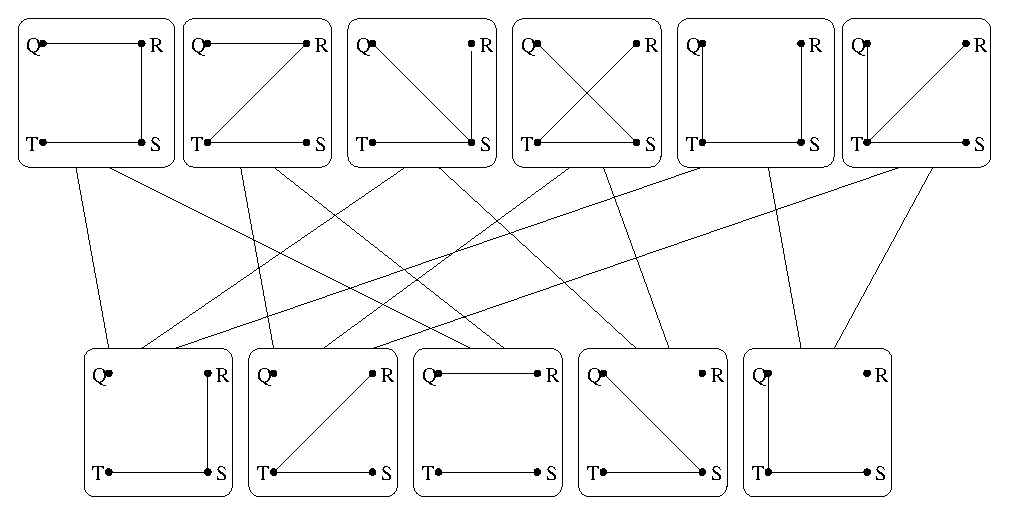
\includegraphics{figures/conn2.eps}
\caption{\label{fi:gc} Illustration of Theorem \ref{th:gc}}
\end{center}
\end{figure}

For the classical case connectivity is known to be evasive
\cite{felsner92complexity}.  If this lower bound is known elsewhere for 
the quantum bounded error setting the author is unaware of it.  It is
not known if this lower bound is asymptotically tight in the bounded
error setting.  It seems reasonable that this bound could be tight,
given the quadratic speedups realized by AND and OR.  Then again it
also seems reasonable that there is no asymptotic speedup as is the
case for MAJORITY and PARITY.

\subsection{Bipartiteness}
\label{sec:bip}

A second fundamental non-trivial monotone graph property is whether a
graph is bipartite.  This graph property is also evasive.

\begin{theorem}
\label{th:nbpt}
$\Omega(V)$ oracle queries are required to decide whether a simple
undirected graph is bipartite.
\end{theorem}

\begin{proof}
We apply Lemma \ref{lm:1xky}, we will only consider simple undirected
graphs with $V \ge 3$.  

Let $x$ be the complete bipartite graph with the first $\left\lfloor
V/2 \right\rfloor$ vertices and second $\left\lceil V/2 \right\rceil$
vertices forming the partitions.  Observe that adding any edge to $x$
results in a non-bipartite graph.  There are
\[
\frac{V(V-1)}{2} - {\left\lfloor\frac{V}{2}\right\rfloor} {\left\lceil\frac{V}{2}\right\rceil} 
= \Theta(V^{2})
\]
such graphs, as there are $V(V-1)/2$ possible edges, $\left\lfloor
V/2\right\rfloor \left\lceil V/2\right\rceil$ of which are in $x$.
Lemma \ref{lm:1xky} implies the lower bound $\Omega(\sqrt{V^{2}}) =
\Omega(V)$.
\end{proof}

If this lower bound is known elsewhere the author is unaware of it.
It is not known if this lower bound is asymptotically tight.  

Having seen two fundamental monotone graph properties with lower
bounds potentially quadratically lower than the classical case it is
tempting to believe these lower bounds are tight and that there is
quadratic speedup in the quantum bounded error model for non-trivial
monotone graph properties.  To see this is not the case we need only
examine the non-trivial monotone graph property analogous to MAJORITY.

\section{No Quantum Extension of the Aanderaa-Karp-Rosenberg Conjecture}
\label{sec:arkbad}

The Aanderaa-Karp-Rosenberg conjecture states that all non-trivial
monotone graph properties are evasive in the classical deterministic
setting.  A natural extension of the Aanderaa-Karp-Rosenberg
Conjecture to quantum computing would conjecture all non-trivial
monotone graph properties have the same query complexity, or at least
the same asymptotic query complexity in the bounded error setting.  To
see that no such extension can hold, observe that the following
non-trivial monotone graph properties can be determined by running the
algorithms for OR, AND, and MAJORITY respectively:

\begin{enumerate}
\item Does the graph have at least 1 edge?
\item Is the graph complete?
\item Does the graph have more than half of all possible edges?
\end{enumerate}

Beals et al.\ provide an $O(V)$ oracle query algorithm for computing
the AND or OR of an $O(V^{2})$ bit oracle string in the bounded error
setting \cite{beals98quantum}, and we have a lower bound of
$\Omega(V)$ oracle queries required to compute them from Section
\ref{sec:AOMP}.  We have a lower bound of $\Omega(V^{2})$ oracle 
queries required to compute the MAJORITY of an $O(V^{2})$ bit oracle
string from Section \ref{sec:AOMP}.  Thus some decision problems for
non-trivial monotone graph properties require $\Theta(V)$ oracle
queries and others $\Theta(V^{2})$ in the bounded error setting, and
there is no extension of the Aanderaa-Karp-Rosenberg conjecture to the
quantum bounded error setting.  This does not come as a complete
surprise, as there are quadratic gaps known between the classically
evasive symmetric functions from Chapter \ref{ch:oracle} in the
quantum bounded error setting.  More disappointing is that there are
graph properties for which the quantum bounded error setting can
provide only constant speedup over the classical case.

\newtheorem{cond}{Condition}[section]
\newtheorem{algoi}{Algorithm}[section]

\chapter{Boolean Functions}
\label{ch:general}

In this chapter we consider increasingly general classes of functions.
We first examine lower bounds for tree functions in Section
\ref{sec:tree} and prove $\Omega(\sqrt[4]{N})$ oracle
queries are required to compute a tree function of $N$ bits.

We define nondeterministic decision tree complexity in Section
\ref{sec:dndtc}.  We then prove that $\Omega(\sqrt{N})$ oracle queries
are required to compute any $N$ bit Boolean function with
nondeterministic decision tree complexity $N$ in Section
\ref{sec:b4r}.  Finally in Section \ref{sec:lqbcbf} we present our
most general result: $\Omega(\sqrt[4]{D(f)})$ oracle queries are
required to compute a class of Boolean functions that meet a
sensitivity condition and have deterministic decision tree complexity
$D(f)$.

\section{Tree Functions}
\label{sec:tree}

Tree functions are Boolean functions of $N$ bits that can be written
as a disjunction of conjunctions in which each of the $N$ variables
occurs exactly once.  Tree functions are evasive in the classical case
\cite{lovasz94evasive}.

\begin{theorem}
\label{theo:treelow}
$\Omega(\sqrt[4]{N})$ oracle queries are required to compute any tree
function of $N$ bits in the bounded error setting.
\end{theorem}

\begin{proof}
For any tree function $f$ let $d$ be the number of terms, and let
$c_{max}$ be the maximum number of variables in any conjunction.

The tree function $f$ has a conjunctive term of size $c_{max}$.  Let
$x$ be the input that gives every variable in that term the value 1,
and every other variable 0, so that $f(x) = 1$.  The inputs attained
by negating one of the $c_{max}$ 1's in $x$ will yield $0$ when
evaluated by $f$.  Lemma \ref{lm:1xky} implies that
$\Omega(\sqrt{c_{max}})$ oracle queries are required to compute $f$.

The tree function $f$ also has $d$ terms.  Let $x$ be the input that
vices the first variable of every term the value 0 and every other
variable the value 1, so that $f(x) = 0$.  The inputs attained by
negating one of the $d$ 0's in $x$ yield $1$ when evaluated by $f$.
Lemma \ref{lm:1xky} now implies that $\Omega(\sqrt{d})$ oracle queries
are required to compute $f$.

Since $d \ge N/c_{max}$, either $c_{max} > \sqrt{N}$ or $d \ge
\sqrt{N}$, and the theorem follows.
\end{proof}

This lower bound is a special case of the $\Omega(\sqrt[4]{D(f)})$
lower bound for monotone functions proved by Beals et al.\
\cite{beals98quantum}, as tree functions are monotone functions with
decision tree complexity $N$.  Here we see for the first time a gap
that is not quadratic with the classical case.  While this lower bound
agrees with the result for monotone functions, the author believes it
is not asymptotically tight.  Whether there is an $\Omega(\sqrt{N})$
lower bound for computing $N$-bit tree functions is an open question.

\section{Nondeterministic Decision Tree Complexity}
\label{sec:dndtc}

In the presentation of the most general results of this thesis we
refer frequently to deterministic and nondeterministic decision tree
complexity, deterministic decision trees were discussed in Section
\ref{subs:ddt}.  Readers familiar with these topics can proceed
directly to Section \ref{sec:b4r}.

Let $f$ be an $N$-bit Boolean function.  We will use the following
definitions of L{\'{a}}szl{\'{o}} Lov{\'{a}}sz and P{\'{e}}ter
G{\'{a}}cs \cite{lovasz94complexity}.

For every input $x$ let $D(f,x)$ denote the minimum number of bits of
$x$ we could be told to convince us that $f(x)$ takes on a particular
value.  For example: $D($OR$,0^{N}) = N$.  If we are told fewer than
$N$ bits of an input are all 0 we can not determine the value of OR
for that input.  For any other input $x \neq 0^{N}$, $D($OR$,x) = 1$,
because we only need to be told that one bit of the input is a 1.  We
are not concerned with how many oracle queries we have to make in the
worst case to determine $f(x)$, but rather how many bits we could be
told in the best case to be sure of the value $f$ takes on $x$.

\begin{defi}
\label{defi:nd0}
$D_{0}(f) = \max\{D(f,x) | f(x) = 0\}$.  $D_{0}(f)$ is the
nondeterministic decision tree complexity of verifying that an input
takes on $0$ when evaluated by $f$.
\end{defi}

\begin{defi}
\label{defi:nd1}
$D_{1}(f) = \max\{D(f,x) | f(x) = 1\}$.  $D_{1}(f)$ is the
nondeterministic decision tree complexity of verifying that an input
takes on $1$ when evaluated by $f$.
\end{defi}

\begin{defi}
\label{defi:ndc}
$N(f) = \max\{D_{0}(f),D_{1}(f)\} = \max_{x}\{D(f,x)\}$.  The
nondeterministic decision tree complexity of computing an $N$-bit
Boolean function $f$ is the maximum of the nondeterministic decision
tree complexities of verifying any input of $f$ takes on one of
$\{0,1\}$.
\end{defi}

\section{Nondeterministically Evasive Functions}
\label{sec:b4r}

With an understanding of decision tree complexity we can now prove a
lower bound on a class of evasive functions.  In analogy to evasive
functions whose deterministic decision tree complexity is $N$ we call
functions with nondeterministic decision tree complexity $N$
\emph{Nondeterministically evasive}.  Every nondeterministically evasive
functions is evasive.

\begin{theorem}
\label{th:b2r}
$\Omega(\sqrt{N})$ oracle queries are required to compute any
nondeterministically evasive $N$-bit Boolean function in the bounded
error setting.
\end{theorem}

\begin{proof}
We will prove that any nondeterministically evasive $N$-bit Boolean
function $f$ has an input $x$ such that for at least half of the
Hamming neighbors of $x$ disagree with $x$ when evaluated by $f$.
Once this is proved the theorem will follow from Lemma \ref{lm:1xky}.

Assume to the contrary that for all inputs $x$ more than half of $x$'s
Hamming neighbors agree with $x$.  Consider any deterministic decision
tree that computes $f$.  Since $D(f) \ge N(f) = N$, there is some path
$P$ of length $N$ in the tree.  Call the variables along this path $a,
b, \ldots , z$, where each label corresponds to a unique number
between 1 and N inclusive.  Let $x_{a}, x_{b}, \ldots , x_{z}$ be the
values of the corresponding bits along the path.  Let us rearrange the
order of the input bits so that $a$ is the first input bit, $b$ is the
second input bit, and $z$ is the $N$th input bit.  Then path $P$ tells
us $f(x_{a}x_{b}\ldots x_{z})$ is either $0$ or $1$, and
$f(x_{a}x_{b}\ldots\overline{x_{z}})$ is the other.  Without loss of
generality let $f(x_{a}x_{b}\ldots x_{z}) = 1$ and
$f(x_{a}x_{b}\ldots\overline{x_{z}}) = 0$.

By the pigeonhole principle, there is some bit $i < N-1$ such that
\[
\begin{array}{ll}
	f(x_{a}x_{b}\ldots x_{i}\ldots x_{z}) = 1 & 	f(x_{a}x_{b}\ldots x_{i} \ldots \overline{x_{z}}) = 0 \\
	f(x_{a}x_{b}\ldots\overline{x_{i}}\ldots x_{z}) = 1 & 	f(x_{a}x_{b}\ldots\overline{x_{i}}\ldots\overline{x_{z}}) = 0 .
\end{array}
\]
However, if this is the case then we do not need to ask about the
$i$th bit on path $P$.  This argument follows for any path of length
$N$ in our deterministic decision tree.  In this case $D_{0}(f)$ and
$D_{1}(f)$ are at most $N-1$.  $N(f)$ is then $N-1$, a contradiction
to the condition that $N(f) = N$.  Therefore our assumption was false,
and there is at least one input $x$ such that at least half of $x$'s
Hamming neighbors yield a different value than $x$ when evaluated by
$f$.  By Lemma \ref{lm:1xky} $\Omega(\sqrt{N})$ oracle queries are
required to compute $f$ in the bounded error setting.
\end{proof}

This proof establishes that nondeterministically evasive functions
have inputs that are sensitive to negation on at least half of their
bits; the result then follows from Lemma \ref{lm:1xky}.  Not all
evasive functions are nondeterministically evasive.  OR is an example
of a nondeterministically evasive function; since Beals et al.\
provide an $O(\sqrt{N})$ algorithm to compute the OR of $N$ bits, this
lower bound is asymptotically tight.

\section{Sensitive Functions}
\label{sec:lqbcbf}

Nearly all the functions discussed so far have been evasive (or
conjectured to be so).  In our final result we consider functions that
are not necessarily evasive.  We call a Boolean function $f$
\emph{sensitive} if for some input $x$, there are $\Omega(N(f))$ Hamming
neighbors $y$ of $x$ such that $f(x) \neq f(y)$.  It is an open
question whether there are any nonsensitive functions.

\begin{theorem}
\label{th:b4r}
$O(\sqrt[4]{D(f)})$ oracle queries are required to compute any
sensitive function $f$ in the bounded error setting.
\end{theorem}

\begin{proof}
By Lemma \ref{lm:1xky}, $\Omega(\sqrt{N(f)})$ oracle queries are
required to compute any sensitive Boolean function. 

Lov{\'{a}}sz and G{\'{a}}cs \cite{lovasz94complexity} proved that
$D(f) \le D_{0}(f) \cdot D_{1}(f)$, and by definition, $N(f) =
\max\{D_{0}(f),D_{1}(f)\}$.  Thus, $N(f) = \Omega(\sqrt{D(f)})$, 
and the theorem follows.
\end{proof}

Beals et al.\ proved $\Omega(\sqrt[6]{D(f)})$ oracle
queries are required to compute any Boolean function in the bounded
error setting, but they suspect that this lower bound is not tight
\cite{beals98quantum}.  An open question is whether there are any 
functions which are not sensitive.  If not, then
$\Omega(\sqrt[4]{D(f)})$ oracle queries are required to compute any
Boolean function, which would be an improvement over what is currently
known.


\chapter{Open Questions}
\label{ch:open}

Ambainis' Theorem has shown itself to be remarkably versatile in
proving lower bounds on Boolean functions; it can frequently be used
to establish asymptotically tight lower bound with little effort.
These lower bounds can be contrasted with classical lower bounds to
see areas where a quantum computer could significantly outperform a
classical computer.  For all the functions we have examined the
separation found between the best known quantum and classical lower
bounds is a polynomial.  Beals et al.\ proved $\Omega(\sqrt[6]{D(f)})$
oracle queries are required to compute an arbitrary Boolean function
$f$ with decision tree complexity $D(f)$ in the bounded error setting
\cite{beals98quantum}.  Therefore there can be no exponential
separation between the classical and quantum oracle query complexity
for Boolean functions.  It should be stressed that this result has
only been proven to hold in the quantum oracle model, only for total
Boolean functions, and only in the bounded error setting (which
includes the exact and zero error settings).

It is suggested by Beals et al.\ that the
$\Omega(\sqrt[6]{D(f)})$ lower bound on the number of
oracle queries required to compute an arbitrary total Boolean function
$f$ is not optimal \cite{beals98quantum}.  It remains an important
open question what the asymptotically tight lower bound is.  In
Section \ref{sec:lqbcbf} we proved $\Omega(\sqrt[4]{D(f)})$
oracle queries are required to compute sensitive Boolean functions, if
the need for sensitivity could be eliminated it would give a better
lower bound than what is currently known.

The importance of quantum computation itself will be quantified by the
speedup allowed by quantum algorithms.  If large classes of useful
problems are found for which a quantum algorithm can provide
exponential speedup, it will certainly drive interest in the
construction of quantum computing devices.  Shor's algorithm currently
stands alone as a useful task that can be performed exponentially
faster by a quantum algorithm than with the best published classical
algorithm.  There are many other problems that show this exponential
separation, but the are toy problems tailored to display such speedup
and have no practical application.

The current uniqueness of Shor's algorithm is a great enticement to
further study.  It is hard to believe that there is only one useful
problem that we can find exponential speedup for; however, results
such as the ones in this thesis seem to indicate that for many
reasonable models of computation only polynomial speedup can be
attained.  In some way this parallels the results of Grover's
algorithm which provides quadratic speedup over what is classically
possible for the unordered search problem, but disallows any potential
exponential speedup by its optimality.

Whether a quantum computer of a size great enough to perform useful
calculations can be built is unclear, but great progress has been
made.  On December 19, 2001, IBM researchers announced they had
factored the number 15 on a quantum computer running Shor's algorithm
\cite{ibm01shor}.  When tempted to prognosticate about the future of
this nascent technology, it is instructive to examine predictions made
around the time of the birth of the digital computer.  In 1949
\emph{Popular Mechanics} boldly posited:
\begin{quote}
Where \ldots the ENIAC is equipped with 18,000 vacuum tubes and
weights 30 tons, computers in the future may have 1,000 vacuum tubes
and perhaps weigh just one and a half tons\cite {patterson98computer}.
\end{quote}
While the future of quantum hardware may be uncertain, a few quantum
algorithms discovered so far are impressive.  The discovery of
fundamental tasks that can be performed quadratically faster in the
bounded error setting than in the classical setting, such as computing
the AND and OR of $N$ bits, promise surprising results for more
interesting problems in the future.


%%\appendix

%%\include{A-data.tex}

\backmatter

\bibliography{thesisbib}
\bibliographystyle{plain}

%%\chapter{Vita}

%%Juan Valdez was born\ldots.

\end{document}
\endinput
%%
%% End of file `thesis-ex.tex'.
